\documentclass[tikz, border=7pt]{standalone}

\usepackage[T1]{fontenc}
\usepackage[english]{babel}

\usepackage{xcolor}

\usepackage{tikz}

\begin{document}
    \begin{tikzpicture}
        \node (lods) at (0,0) {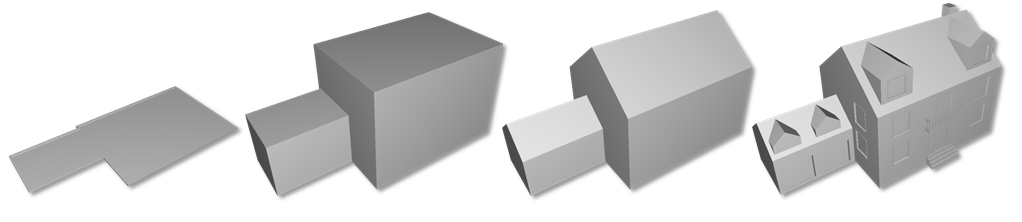
\includegraphics[height=10em]{images/lods}};
        \path (lods.south) + (-6,0) node (lod0) {\textbf{LoD-0}};
        \path (lods.south) + (-2,0) node (lod0) {\textbf{LoD-1}};
        \path (lods.south) + (2,0) node (lod0) {\textbf{LoD-2}};
        \path (lods.south) + (6,0) node (lod0) {\textbf{LoD-3}};
    \end{tikzpicture}
\end{document}